\section{Selection}

\subsection{Dataset}
This analysis uses all the \pp collision data in Run 1 and Run 2 stage, 
corresponding to an integrated luminosity of $3\invfb$ ($6\invfb)$ in Run 1 (Run 2).
The simulation samples of the $\LbJpsiPPi$ decay are generated by \pythia with $pp$ collisions at $\sqrt{s}=7\tev$, $8\tev$ and $13\tev$ respectively,
with the ratio of the numbers of events roughly one to two between Run 1 and Run 2.
Both \pythia6 and \pythia8 generators are used.
The Monte Carlo event type is \texttt{15144021}, 
in which $\Lb$ is forced to decay into the $\jpsi\proton\pim$ final state with the PHSP model.

%
\subsection{Reconstruction and pre-selection}
In this analysis the reconstruction of the \Lb candidate starts
from the stripping line \texttt{FullDSTDiMuonJpsi2MuMuDetachedLine} in the \texttt{DiMuon} stream 
of the stripping reconstruction,
which different version, 
\texttt{S21} for 2011, 
\texttt{S21r1} for 2012, 
\texttt{S24} for 2015, 
\texttt{S28} for 2016, 
\texttt{S29r2} for 2017, 
and \texttt{S34} for 2018. 
The selection criteria in this stripping line is summarized in Table~\ref{tab:JpsiSelection}.
The \jpsi candidate is formed by two oppositely charged tracks consistent with muon hypotheses (IsMuon) 
with $\pt>550\mevc$ and good track fit quality $\chisqndf<4$.
The $\jpsi$ candidate is required to have an invariant mass within the $\pm100\mevcc$ window 
around the know \jpsi mass~\supercite{PDG2014}, and to have a vertex fit quality $\chisqvtx<20$.
The $\jpsi$ candidate is consistent with originating from $b$-hadron decays by requiring its decay length significance (DLS) to be greater than three.

%
Conparing to the previous study\supercite{LHCb-PAPER-2016-015},
the selection criteria is optimized,
all differences between the new selection criteria and old study are summarized in Table~\ref{tab:PreSelection}.
To select good $\jpsi$ candidates,
a tightened PID cut $\dllmupi>0$ is required for both muon tracks in the final state,
and the dimuon invariant mass window is reduced to $[-48,\,43]\mevcc$ around the known \jpsi mass~\supercite{PDG2020}.
The \jpsi mass resolution is around $13\mevcc$.
To reconstruction the \Lb candidate, 
the $\jpsi$ candidate is combined with two opposite charged tracks, 
consistent with pions and protons respectively.
This is achieved by PID cuts on the \ProbNN variables: $\ProbNN_{\pi}(\pi)>0.2$ and $\ProbNN_{p}(p)>0.2$.
%The proton is required to have large momentum, $p>10\gevc$,
%in order to keep the power of discriminating protons against kaon misidentification,
%and the good performance of the PID calibration.
%For similar reason (could also remove background) the momentum of the $\pi$ is required to be larger than $3\gevc$.
The two hadronic tracks are required to have large transverse momenta, $\pt>250\mevc$,
inconsistent with originating from the primary vertex (PV), $\chisqip>9$.
%The $\Lb$ candidate is required to have a displayed decay vertex, $\chisq_\tau>9$, with good vertex fit quality, $\chisqndf<10$.
The $\Lb$ candidate is required to have a good vertex fit quality, $\chisqndf<10$, 
with a displayed decay vertex,
flight distance to primary vertex is larger than $1.5$\mm.
It should be consistent with being produced from PV by requiring $\chisqip<25$ and cosine value of the direction angle, DIRA$>0.999$.
And the \chisq of closet approach distance between \proton and \pim is smaller than 20.
The $\Lb$ candidates with mass $5.1<M(\jpsi p\pi^-)<6.5 \gevcc$ are selected.

The $\LbJpsiPPi$ decay chain is refitted with two sequential constraints using the \texttt{DecayTreeFitter} to improve the mass resolution:
A) the \jpsi candidate mass constrained to its known value~\supercite{PDG2020} and
the $\Lb$ candidate constrained to originating from the PV;
B) the invariant mass of the $\Lb$ candidate constrained to its know value~\supercite{PDG},
with the momenta of the $\jpsi$, $p$ and $\pim$ daughters re-calculated according to this constraint.

It should be noted that the PID requirements on the hadron tracks are not applied when reconstructing the $\Lb$ candidates in the simulation sample.
The effect, instead, is considered using weights from the PID calibration (\texttt{PIDCalib}).
The pion track is calibrated using pion tracks from the $\Dstar$ tagged $\decay{\Dz}{\Km\pip}$ decay, 
while the proton track is calibrated using proton tracks from the $\decay{\Lc}{p\Km\pip}$ decay.

Events with $\Lb$ candidates in both the simulation and the data samples are required to fire (TOS) the trigger sequences: 
%at the \lone level by either of the \texttt{L0Muon} and \texttt{L0DiMuon} lines; 
at the \hltone level by either of the \texttt{Hlt1DiMuonHighMass}, \texttt{Hlt1TrackMuon}, \texttt{Hlt1TrackMVADecision} 
and \texttt{Hlt1TwoTrackMVADecision} lines; 
and at the \hlttwo level by either of
the \texttt{Hlt2DiMuonDetachedJPsi} and \texttt{Hlt2TopoMu(2,3,4)BodyBBDT} lines.


%Reflections of $\Bz$ and $\Bs$ decays are determined by changing the particle hypotheses of the hadron tracks, 
%and re-calculating the invariant mass under the constraint A.

%%%%%%%%%%%%%%%%%%%%%%%%%%%%%%%%%%%%%%%%%%%%%%%%%%%%%%%%%%%%%%%%%%%%%%%%%%%%%%%%%%%%%%%%%%%%%%%%%%%%%%%%%%%%%%%%%%%%%%%
\begin{table}[tbh]
\caption{Stripping selections of $\jpsi$ candidates in the line \texttt{FullDSTDiMuonJpsi2MuMuDetachedLine}.}
\centering
\begin{tabular}{rl}
\hline
Quantity               & Selections \\
\hline
IsMuon$(\mu)$          & $=$ TRUE \\
DLL$(\mu-\pi)$     & $>$ 0\\
$\pt(\mu)$             & $>550\mevc$ \\
Track $\chisqndf(\mu)$ & $<4$  \\
$\Delta M(\jpsi)$      & $<100\mevcc$\\
Vertex $\chisq(\jpsi)$ & $<20$ \\
DLS($\jpsi$)           & $>3$  \\
\hline
\end{tabular}
\label{tab:JpsiSelection}
\end{table}
%%%%%%%%%%%%%%%%%%%%%%%%%%%%%%%%%%%%%%%%%%%%%%%%%%%%%%%%%%%%%%%%%%%%%%%%%%%%%%%%%%%%%%%%%%%%%%%%%%%%%%%%%%%%%%%%%%%%%%%

%%%%%%%%%%%%%%%%%%%%%%%%%%%%%%%%%%%%%%%%%%%%%%%%%%%%%%%%%%%%%%%%%%%%%%%%%%%%%%%%%%%%%%%%%%%%%%%%%%%%%%%%%%%%%%%%%%%%%%%
%\begin{table}[tbh]
%\caption{Pre-selections of $\LbJpsiPPi$ candidates.}
%\centering
%\begin{tabular}{rl}
%\hline
%Quantity                & Selections  \\
%\hline
%$\ProbNNp(p)$           & $>0.1$ \\
%$P(p)$                  & $>10\gevc$ \\
%$\ProbNN_{\pi}(\pi)$    & $>0.05$ \\
%$\pt(p,\pi)$            & $>250\mevc$ \\
%$\chisqip(p,\pi)$       & $>9$ \\
%Vertex $\chisqndf(\Lb)$ & $<10$   \\
%$\chisq_{\tau}(\Lb)$    & $>9$   \\
%$\chisqip(\Lb)$         & $<25$   \\
%DIRA$(\Lb)$             & $>0.9995$   \\
%$M(\jpsi\proton\pim)$   & $\in[5.1,6.5]\gevcc$   \\
%\hline
%\end{tabular}
%\label{tab:PreSelection}
%\end{table}


\begin{table}[tbh]
\caption{Pre-selections of $\LbJpsiPPi$ candidates between old Run 1 analysis and this one.}
\centering
\begin{tabular}{c c | c c}
\hline
    & Quantity               & Old Run 1 & This analysis \\
\hline
1   & All tracks \chisqndf   & $<3$      		& same  \\
2   & muon DLL(\muon)        & $>0$\&ISMUON	& same  \\
3   & \pt of muon   	     & $>550\mev$      	& same  \\
4   & \pt of hadron	     & $>250\mev$      	& same  \\
5   & vertex of \jpsi        & $\chisq<16$      & same  \\
6   & mass window of\jpsi    & $[-48,43]\mev$   & same  \\
7   & \chisqvs of hadron     & $>9$      		& same  \\
8   & PID of $\pi$   	     & ProbNNpi$\times$(1-ProbNNpi)$>0.5$      	& ProbNNpi$>0.2$  \\
9   & PID of \proton   	     & ProbNNpi$>0.1$   				& ProbNNpi$>0.2$  \\
10   & \chisqip of \Lb    	& $<25$      		& same  \\
11   & \Lb vertex   		& $\chisqvtxndf<10$     & same  \\
12   & DIRA of \Lb   		& $>0.9995$      		& $>0.999$ \\
13   & $\chisq_{\tau}$ of \Lb  	& $>9$      	& -  \\
14   & \ptot(\proton)   		& $>10\gev$       & -  \\
15   & Flight distance of \Lb	   	& -      		& $>1.5\mm$ \\
16   & DOCA \chisq of \proton\pim   & -      		& $<20$ \\
%17   & Clone track		   	& -      		& GhostProb$<0.2$ \\
\hline
\end{tabular}
\label{tab:PreSelection}
\end{table}
%%%%%%%%%%%%%%%%%%%%%%%%%%%%%%%%%%%%%%%%%%%%%%%%%%%%%%%%%%%%%%%%%%%%%%%%%%%%%%%%%%%%%%%%%%%%%%%%%%%%%%%%%%%%%%%%%%%%%%%

%
\subsection{Reflections vetoing}
%Since the decays of $\Bd\to\jpsi K\pi$, $\Bs\to\jpsi K K$, $\B^0_{(\squark)}\to\jpsi\pi\pi$, 
Since the decays of $\Bd\to\jpsi K\pi$, $\Bs\to\jpsi\Kp\Km$, 
$\LbJpsipK$ have much larger branching fractions than the \LbJpsippi decay,
even after the PID requirements on the hadron tracks,
the \LbJpsippi sample is still potentially contaminated by these decays.
To investigate the effects of the reflections from these decays,
the invariant mass of the \Lb candidate in the \LbJpsippi sample is re-calculated
with the proton assumed as a pion or kaon and/or the pion assumed as a kaon or proton.
Figure~\ref{fig:Reflections} shows 
these re-calculated invariant mass distributions for those \LbJpsippi candidates 
within the $\pm20\mevcc$ mass window ($\approx3\sigma)$) around the known \Lb mass\supercite{PDG2020}.
Clear contamination with the $\Bd\to\jpsi K\pi$, $\Bs\to\jpsi K K$ and $\LbJpsipK$ decays are observed, 
as shown by the narrow peaks around the known $\Bd$, $\Bs$ and $\Lb$ masses in the top right, 
bottom left and bottom middle plots in Fig.~\ref{fig:Reflections}.
The contribution of $B^0_{(\squark)}\to\jpsi\pi\pi$ decays is insignificant.
The contamination from $\Bd\to\jpsi K\pi$ is vetoed if:
$M(\jpsi [\proton\to K]\pi)$ sits in the $\pm22\mevcc$ window around the known $\Bz$ mass\supercite{PDG2020},
or $M(\jpsi [\proton\to\pi][\pi\to K])$ sits in the $\pm22\mevcc$ window around the known $\Bz$ mass 
and ProbNNpi(\proton)$>0.1$\&ProbNNk($\pi$)$>0.1$.
The contamination with the \LbJpsipK decay is vetoed if:
$M(\jpsi \proton[\pim\to K])$ sits in the $\pm22\mevcc$ window around the known $\Lb$ mass\supercite{PDG2020} 
and ProbNNk($\pi$)$>0.2$,
or $M(\jpsi [\proton\to K][\pi\to\proton])$ sits in the $\pm22\mevcc$ window around the known $\Bz$ mass 
and ProbNNk(\proton)$>0.1$\&ProbNNp($\pi$)$>0.1$.
Besides, 
the reflection of $\Bs\to\jpsi\Kp\Km$ decay is removed in this case: 
$M(\jpsi [\proton\to K][\pim\to K])$ sits in the $\pm22\mevcc$ window around the known $\Bs$ mass\supercite{PDG2020}.

%The contamination with these decays are suppressed by invariant mass vetoes:
%Events are removed from the \LbJpsippi sample, 
%if $M(\jpsi K\pi)$ sits in the $\pm21.8\mevcc$ window around the known $\Bz$ mass\cite{PDG2020}, 
%or $M(\jpsi KK)$ sits in the $\pm19.3\mevcc$ window around the known $\Bs$ PDG mass.
%Both values correspond to three times of the mass resolutions.
%The contamination with the \LbJpsipK decay is not vetoed because 
%1) the effect is small and 
%2) the efficiency due to this veto is very small.
%Instead, 
%the reflection of the \LbJpsipK decay is taken into account in the \LbJpsippi invariant mass distribution, 
%and the shape is determined from simulation.
%Besides, 
%the $\decay{\Lb}{\jpsi p K}$ decay, 
%when the $K$ is reconstructed as a $\pi$, 
%locates in the left sideband of the signal region, 
%and its shape is also determined from simulation.

A large fraction of \LbJpsippi candidates come from the decay $\decay{\Lb}{\jpsi\Lambda^0}$ with $\decay{\Lambda^0}{p\pi^-}$, 
which is not interesting in this analysis.
These events are removed if the invariant mass $M(p\pim)$ locates in the $\pm 5\mevcc$ window around the known $\Lambda^0$ mass~\supercite{PDG2020}.

During the invariant mass vetoing, 
the mass resolutions are determined by fitting the invariant mass distribution in a narrow region around the signal peak; 
the signal mass shape is described by double-sided crystal ball function (DSCB) with tail parameters fixed to
the $\LbJpsiPPi$ simulation, 
while the background is simply described by a linear function.

%%%%%%%%%%%%%%%%%%%%%%%%%%%%%%%%%%%%%%%%%%%%%%%%%%%%%%%%%%%%%%%%%%%%%%%%%%%%%%%%%%%%%%%%%%%%%%%%%%%%%%%%%%%%%%%%%%%%%%%
\begin{figure}[!tbh]
\centering
\begin{minipage}[t]{1.0\textwidth}
\centering
\includegraphics[width=0.3\textwidth]{Figures/04_Penta/02_selection/draw_veto_pic/Lb_mass_P2K}
\includegraphics[width=0.3\textwidth]{Figures/04_Penta/02_selection/draw_veto_pic/Lb_mass_P2Pi}
\includegraphics[width=0.3\textwidth]{Figures/04_Penta/02_selection/draw_veto_pic/Lb_mass_PPi2KK} \\
\includegraphics[width=0.3\textwidth]{Figures/04_Penta/02_selection/draw_veto_pic/Lb_mass_PPi2KP}
\includegraphics[width=0.3\textwidth]{Figures/04_Penta/02_selection/draw_veto_pic/Lb_mass_PPi2PiK}
%\includegraphics[width=0.3\textwidth]{Figures/04_Penta/02_selection/draw_veto_pic/Lb_mass_PPi2PiP} \\
\includegraphics[width=0.3\textwidth]{Figures/04_Penta/02_selection/draw_veto_pic/Lb_mass_Pi2K} 
   %\put(-120,230) {\textrm{\small\bf {LHCb Unofficial} }}\\
   %\put(-120,230) {\textrm{\small \bf \color{red}{ LHCb Unofficial} }}\\
\end{minipage}
\caption{
  Invariant mass distributions of the \LbJpsippi candidate with the $p$ and the $\pim$ assumed to be other hadrons 
   for those \Lb candidates in the $\pm20\mevcc$ mass window around the know \Lb mass.
  The lablels $\hadron\to\hadron'$ indicate that the \hadron hadron in the \LbJpsippi decay is assumed as a $\hadron'$ hadron.
}
\label{fig:Reflections}
\end{figure}
%%%%%%%%%%%%%%%%%%%%%%%%%%%%%%%%%%%%%%%%%%%%%%%%%%%%%%%%%%%%%%%%%%%%%%%%%%%%%%%%%%%%%%%%%%%%%%%%%%%%%%%%%%%%%%%%%%%%%%%



\subsection{Multivariate analysis}

The multivariate analysis (MVA) is used to further suppress the background. 
In the MVA training the signal sample is from the $\LbJpsiPPi$ simulation using the PHSP model, 
while the background sample is from the upper sideband of the $\LbJpsiPPi$ invariant mass distribution, 
$M(\jpsi p\pi)\in[5.67,5.80]\gevcc$.
These samples are randomly split into two halves, one for the training and the other for the test.
Different from the previous study,
the PID information variables are included in the MVA classification.
All used variables are listed it Table.~\ref{tab:MVA}
The smaller value of the two muon PID variables ($\dllmupi$);
the smaller value of the $\chisqip$ of the two muon tracks;
the smaller value of the $\chisqip$ of the two hadron tracks;
the arithmetic addition of the \pt of the two hadrons;
the DIRA, the flight distance (FD), the $\pt$, the $\chisqip$ and the vertex fit quality ($\chisqvtxndf$) of the $\Lb$ candidate.
the PID varibles of hadrons.
Besides,
the Run 1 and Run 2 samples are studied seperately.
The distributions of these variables of Run 1 sample for the signal in the simulation sample and the background in the data sideband 
are shown in Figure.~\ref{fig:MVAvairables},
corresponding Run 2 distributions are shown in Appendix.~\ref{}.

\begin{table}[tbh]
\caption{Variables used in TMA between previous Run1 and this study.}
\centering
\begin{tabular}{c | c | c }
\hline
    & Previous Run 1   	     & This analysis \\
\hline
1   & \chisqvtx of \Lb       & same  \\
2   & sum \pt of hadrons     & same  \\
3   & \chisqip of \Lb        & same  \\
4   & DIRA of \Lb	           & same  \\
5   & min \chisqip of hadrons& same  \\
6   & min \chisqip of muon   & same  \\
7   & FD of \Lb              & same  \\
8   & \pt of \Lb   	     & same  \\
9   & min PID of muon        & same  \\
10   & -       	 	     & ProbNNp of \proton  \\
11   & -   	     		     & ProbNNpi of \pim  \\
12   & -   	     		     & momentum of \proton \\
\hline
\end{tabular}
\label{tab:MVA}
\end{table}

\begin{figure}[!tbh]
\centering
\begin{minipage}[t]{1.0\textwidth}
\centering
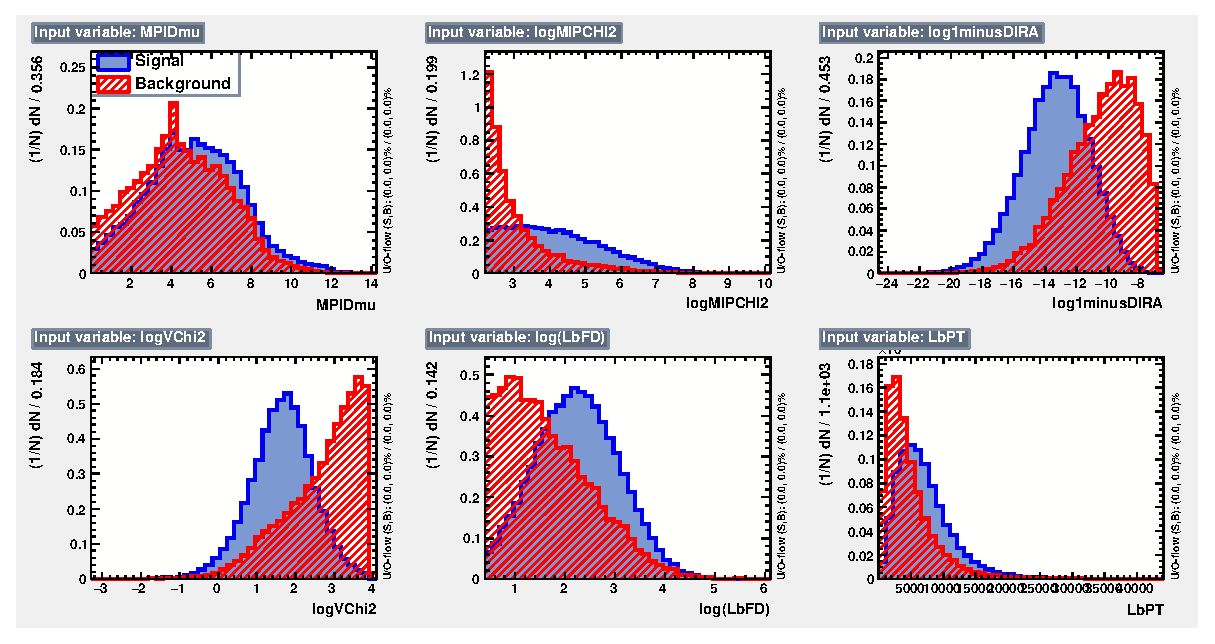
\includegraphics[width=0.95\textwidth]{Figures/04_Penta/02_selection/tmva/plots_run1/variables_id_c1} \\
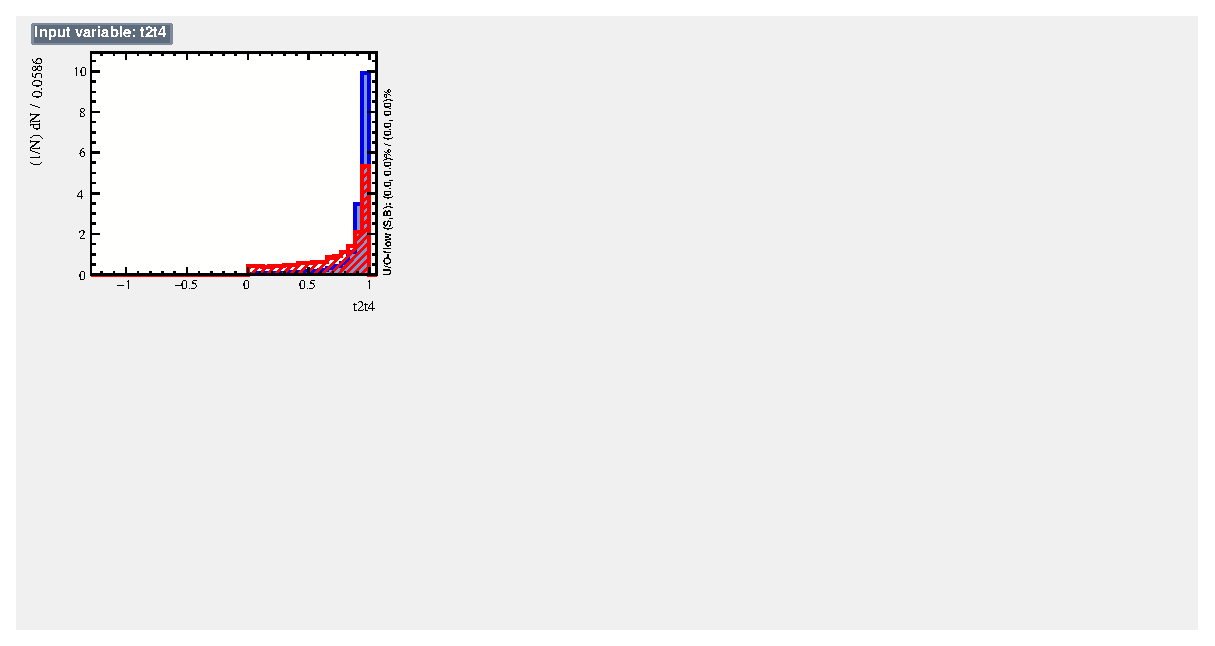
\includegraphics[width=0.95\textwidth]{Figures/04_Penta/02_selection/tmva/plots_run1/variables_id_c2}
\end{minipage}
\caption{Discriminating variables used in the MVA training of Run 1 sample.}
\label{fig:MVAvairables}
\end{figure}

%The ROC curves of the results of different training methods are given in the left plot of Fig.~\ref{fig:MVAMonitor}.
The BDTG method is used as the default method, 
and the overtraining test for the BDTG method is given in the right plot of Figure.~\ref{fig:MVAMonitor} for both Run 1 and Run2 samples.
The BDTG discriminant distributions for the training samples are consistent with those in the test samples. 
No effect of overtraining is observed.
The working point of the BDTG value is optimized by maximizing the figure of merit (FoM) of the signal significance, 
defined as $\epsilon_S/\sqrt{S+B}$.
The $\epsilon_S$ is the signal efficiency for a specified BDTG cut and is determined from the simulation sample, 
while $S$ ($B$) is the number of the signal (background) events in the $\pm3\sigma$ region around the known $\Lb$ mass 
in the $\jpsi\proton\pi$ invariant mass distribution of the data.
%It should be noted that the PID requirements on the $p$ and $\pi$ need also to be tightened on top of the pre-selection.
%However, 
%it is found that the BDTG cut value that maximizes the FoM doesn't depends strongly on the PID cuts of the two hadron tracks.
In Figure.~\ref{fig:BDTGCut}, 
the distribution of the FoM as a function of the BDTG cut value is given, 
and the value of $0.88$ for Run 1 and $0.9$ for Run 2 are determined as the default working points.

%The PID requirement on the proton is tightened slightly to $\ProbNN_p>0.2$ 
%to further suppress the background and retain a high efficiency of the signal selection.
%Because it is found that tighter requirement will reduce significant amount of signals,
%so no tighter requirement is applied on the proton PID. 
%The PID requirement on the $\pi$ track is efficient to suppress the CKM favoured decay \LbJpsipK, which is an avoidable background component.
%A cut on the combined PID variable, $\ProbNN_{\pi}\times(1-\ProbNN_{K})>0.5$ is applied to the $\pi$ track, 
%which suppresses the background to a reasonable level, 
%and leaves about $90\%$ of the signals on top of the pre-selection. 
%The efficiency of the additional PID requirements is about $81\%$ for signals.


%%%%%%%%%%%%%%%%%%%%%%%%%%%%%%%%%%%%%%%%%%%%%%%%%%%%%%%%%%%%%%%%%%%%%%%%%%%%%%%%%%%%%%%%%%%%%%%%%%%%%%%%%%%%%%%%%%%%%%%
\begin{figure}[!tbh]
\centering
\includegraphics[width=0.48\textwidth]{Figures/04_Penta/02_selection/tmva/plots_run1/overtrain_BDTG}
\includegraphics[width=0.48\textwidth]{Figures/04_Penta/02_selection/tmva/plots_run2/overtrain_BDTG}
\caption{
   The BDTG output distribution for signals and the background in the training sample and the test sample of Run 1(left) and Run 2(right) samples.}
\label{fig:MVAMonitor}
\end{figure}

\begin{figure}[!tbh]
\centering
\includegraphics[width=0.48\textwidth]{Figures/04_Penta/02_selection/tmva/plots_run1/mvaeffs_BDTG}
\includegraphics[width=0.48\textwidth]{Figures/04_Penta/02_selection/tmva/plots_run2/mvaeffs_BDTG}
   \caption{Signal significance (arbitrary unit) for different BDTG cut values of Run 1(left) and Run 2(right) samples.}
\label{fig:BDTGCut}
\end{figure}
%%%%%%%%%%%%%%%%%%%%%%%%%%%%%%%%%%%%%%%%%%%%%%%%%%%%%%%%%%%%%%%%%%%%%%%%%%%%%%%%%%%%%%%%%%%%%%%%%%%%%%%%%%%%%%%%%%%%%%%



%\subsection{Comparison of selections with those in $\Lb\to\jpsi pK$ analysis}
%\label{subsec:cmp}
%The two analyses use the same stripping line \texttt{Jpsi2MuMuDetachedLine} to reconstruct and select the $\jpsi$ candidates. T
%he pre-selections in the two analysis are very similar, except that
%\begin{itemize}
%\item DIRA$(\Lb)>0.9995$ instead of
%DIRA$(\Lb)>0.999$, which is still loose enough for signals and will be used in further MVA to be tightened, so should be fine,
%\item this analysis also uses Hlt2
%topological triggers, and since these lines have large overlap with the DetachedJpsiLine for the decay in these two
%analyses, and are developed
%dedicated for $b$-hadron decays and commonly used and should also be fine,
%\item we require also TOS at L0 stage on the
%muon lines, since we do this on both simulation and data, and simulation is justified to be good enough in describing
%muon triggers, these requirements are not problems.
%\item in  $\Lb\to\jpsi pK$ analysis the pre-selection requires flight distance of $\Lb$ to be larger than $1.5\mm$,
%while this analysis requires lifetime significance of $\Lb$ to be larger than 9. The two selections are highly
%correlated. Besides, the flight distance variable will be used in MVA analysis, and the cut in pre-selection will be
%overwritten.
%\item among the nine variables in the MVA training, eight of them are the same except that we added IP chi2 $\chisqip$ of the
%muons in parallel to the hadrons. This also should not be a problem, since the variable is related to $\Lb$ lifetime,
%      which is the main selection criteria of these analyses.
%\item the PID selections are quite different due to the fact that the channel in this analysis is a CKM suppressed
%one relative to $\Lb\to\jpsi pK$. So we apply tighter cuts on the pion to suppress the CKM favored $\Lb\to\jpsi pK$ background. We don't apply
%tight cut on the proton since it is not efficient to improve the signal-to-background ratio concerning the reflection
%peaking background this analysis, instead we apply vetos to remove the peaking background almost completely. The PID
%selection efficiency thus keeps very high of around $87\%$.
%\item the $B\to \jpsi hh$ decays have much larger branching fraction, so would be difficulty for this analysis to
%model them in the invariant mass, so we have to make the vetos on these reflections. While in $\Lb\to\jpsi pK$ analysis,
%      the reflections are relatively smaller in yields, and thus can be easily reduced to a negligible level by the PID,
%      so the vetos are not required.
%\end{itemize}







